\chapter{Entorno virtual}

% **************************** Define Graphics Path **************************
\graphicspath{{Chapter3/Figs/}}

Uno de los principales objetivos de este trabajo es realizar pruebas funcionales y de escala sobre la arquitectura del prototipo. Es de interés generar distintas realidades, y así detectar puntos de falla o variables clave en el rendimiento de la arquitectura. Para modelar las distintas realidades se puede utilizar dos parámetros: topología y servicios. Es importante poder aplicar topologias complejas y relativamente grandes a la arquitectura, así como grandes cantidades de servicios, y de esta forma encontrar posibles problemas con la arquitectura, y su respectiva solución. Dado que no es realista hacer este tipo de pruebas con un prototipo físico, por temas económicos y prácticos, se observa la necesidad de un entorno virtual capaz de simular las características del prototipo. Es importante remarcar que también tendría un gran valor como herramienta de investigación, para trabajar sobre la arquitectura de RAUFlow pero también para futuros estudios sobre esquemas híbridos SDN/Legacy. \\
En este capítulo se estudian los requerimientos que debe cumplir este entorno y los detalles de diseño e implementación de la solución construida. También se explican los principales problemas o dificultades encontradas para lograr un correcto funcionamiento, así como el desarrollo de un módulo que permite cargar topologias automáticamente desde archivos con formato GraphML.

\section{Requerimientos del entorno virtual}
El primer paso en la construcción del entorno virtual es analizar cómo debería comportarse. Se podría hacer este análisis en dos partes separadas. En primer lugar, se deben cumplir los aspectos funcionales de la arquitectura de RAUFlow. No es un requerimiento que se utilicen las mismas herramientas que utiliza el prototipo físico pero es deseable que así sea. Cuanto más similar sea el entorno a la arquitectura, más relevantes serán las pruebas que se lleven a cabo. Otra ventaja es que se pueden reutilizar recursos, como por ejemplo, archivos de configuración. Este primer grupo de requerimientos se detalla a continuación.

\begin{enumerate}
	\item Se debe poder simular múltiples RAUSwitch virtuales, y los mismos deben tener las mismas capacidades funcionales que sus pares físicos. A partir de esto, se desprenden los siguientes sub-requerimientos.
	\begin{enumerate}
		\item Deben poder utilizar el protocolo de enrutamiento OSPF. Esto es necesario ya que la base de datos topológica de RAUFlow se construye a partir de la base de datos local de OSPF (Link-State Database).  Es deseable que lo hagan mediante el software de enrutamiento Quagga.
		\item Resulta trivial que los RAUSwitch virtuales soporten OpenFlow, ya que es el cimiento de RAUFlow. Específicamente, deben soportar la versión 1.3. Esto se debe a que la implementación de las VPNs depende de que los nodos tengan soporte para MPLS, y OpenFlow ofrece esta funcionalidad de forma completa a partir de la versión 1.3. Es muy deseable que lo hagan mediante Open vSwitch, ya que es la herramienta utilizada por los RAUSwitch físicos.
		\item En la arquitectura de RAUFlow se usan agentes SNMP para que los RAUSwitch envíen información que no es soportada por el protocolo OpenFlow acerca de sus interfaces. Como requerimiento para este entorno, es importante que los nodos puedan enviar esa información de algún modo, pero no es necesario que sea a través de SNMP, ya que no es una parte vital de la arquitectura.
	\end{enumerate}
	\item Se debe poder simular múltiples hosts, ya que son los agentes que se conectan a la red y utilizan la misma para enviarse datos entre sí. De esta forma se corrobora que el funcionamiento de la red es el correcto.
	\item La aplicación RAUFlow debe ejecutarse y comunicarse correctamente con los RAUSwitch. Esto también implica que el controlador Ryu debe ser soportado por el entorno. \\

En el segundo grupo de requerimientos, se consideran los que son inherentes a cualquier herramienta de virtualización que se utilizará para pruebas de escala como las que se pretenden.
 
	\item Facilidad de configuración. Es importante que el entorno pueda generar distintas topologias y escenarios sin demasiado esfuerzo de configuración.
	\item Escalabilidad. El entorno debería ofrecer buena escalabilidad en la cantidad de nodos que puede simular. Esto se traduce a que una computadora promedio de uso personal pueda levantar algunas decenas de nodos virtuales como mínimo.
\end{enumerate}

\section{Elección de la herramienta}
Teniendo definidos los requerimientos, el siguiente paso es obtener una herramienta de virtualización que cumpla dichos requerimientos. Se descarta una construcción "desde cero" de la misma, ya que se considera un esfuerzo demasiado grande para el alcance de este trabajo. Por lo tanto, se debe utilizar una herramienta existente. En el capítulo 2 se presentó un estudio del estado del arte de los emuladores y simuladores de red disponibles en la actualidad. La tabla \ref{table:emuladores-y-simuladores} muestra todas las herramientas estudiadas, y se las puede separar en dos grupos: las orientadas específicamente para SDN y las de propósito general. Muchas de las orientadas a SDN fallan en requerimientos básicos, como la versión de OpenFlow o poder utilizar un controlador personalizado (requerimientos 1.b y 3), y por lo tanto se descartan. Por otro lado, Mininet cumple todos los requerimientos excepto el relacionado al enfoque híbrido (el 1.a) ya que es una herramienta diseñada para el paradigma SDN puro y sus switches no soportan los protocolos IP legados.

Otra opción podría ser utilizar una de las herramientas de propósito general, como IMUNES. Ese tipo de enfoque tiene la ventaja de que los aspectos funcionales (requerimientos 1-3) no son un problema. Esto se debe a que al ser herramientas de propósito general, en definitiva lo que proveen son nodos virtuales Linux genéricos. Por lo tanto se podría replicar lo hecho en los nodos físicos del prototipo en dichas máquinas virtuales. 
El problema de esa opción radica en los últimos dos requerimientos (4 y 5). En primer lugar, muchas de esas herramientas no tienen formas fáciles y rápidas de configurar distintas topologias. En segundo lugar, la escalabilidad de esas herramientas puede ser una limitación. En particular, las herramientas que utilizan máquinas virtuales completas no son un buena opción, ya que cada nodo necesita demasiados recursos de cómputo y no sería viable hacer experimentos de escala. Podrían ser viables las que utilizan virtualización ligera (o basada en containers) ya que cada nodo virtual utiliza menos recursos.

Tomando todo esto en cuenta, la herramienta que se elije para construir el entorno es Mininet, pero de un modo no tradicional. Como se explica en el capítulo 2, Mininet, además de ofrecer switches, ofrece hosts que son containers reducidos. Por lo tanto, la solución que se propone es utilizar a Mininet como emulador de propósito general y basarse en dichos hosts para construir los RAUSwitch virtuales. De este modo, tomando como base lo hecho para los nodos físicos se cubren los requerimientos funcionales, y también se aprovecha la configurabilidad y escalabilidad de Mininet.

\section{Diseño e implementación del entorno}
Como explica la sección anterior, el entorno está construido alrededor de Mininet, y se podría pensar como una extensión de la misma. \textit{Out of the box}, Mininet ya cumple la mayoría de los requerimientos estudiados anteriormente. Está diseñada para ser escalable, ya que usa containers reducidos, tiene soporte para OpenFlow 1.3 mediante Open vSwitch, y gracias a su API en Python es muy fácil de configurar. El aspecto en el que falla es en el soporte para Quagga. Dado que Mininet es una herramienta de prototipado para SDN puro, no está pensado para un esquema híbrido como el que se propone. Los switches compatibles con Open vSwitch que ofrece no pueden tener su propio network namespace, por lo tanto, no pueden tener su propia tabla de ruteo ni interfaces de red aisladas, así que no es posible que utilicen Quagga.

Por otro lado, los hosts de Mininet sí tienen su propio network namespace, y gracias a su capacidad de tener sus propios procesos y directorios, es posible ejecutar una instancia de Quagga y Open vSwitch para cada host. De esta forma es posible convertir un host en un RAUSwitch como el requerido por la arquitectura. Esta extensión de las funcionalidades de los hosts es posible ya que Mininet está programado con orientación a objetos y permite al usuario crear subclases propias de las clases que vienen por defecto. En la figura \ref{fig:clases_entorno} se puede ver la estructura de clases del entorno construido. En las siguientes secciones se procederá a estudiar cada una de ellas.

\begin{figure}[t]
	\caption{Diagrama de clases del entorno.}
	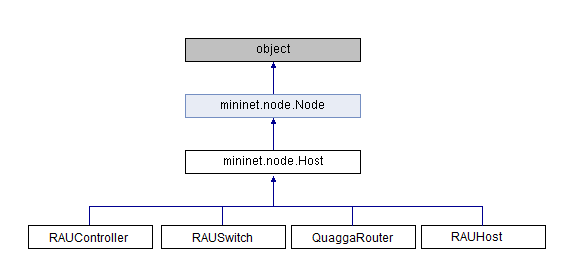
\includegraphics[scale=0.65]{clases_entorno}
	\centering
	\label{fig:clases_entorno}
\end{figure}

\subsection{RAUSwitch}
%mirar http://netgroup.uniroma2.it/twiki/pub/Oshi/WebHome/OSHI_tech_report.pdf pagina 41
La clase RAUSwitch es el núcleo del entorno virtual. Es un Host extendido de tal forma para que, gracias a la funcionalidad de directorios privados, ejecute su propia instancia de Quagga y Open vSwitch. Cada RAUSwitch tiene los siguientes directorios privados: /var/log/, /var/log/quagga, /var/run, /var/run/quagga, /var/run/openvswitch. Cada RAUSwitch también usa un directorio bajo /tmp, para almacenar sus archivos de configuración.

Open vSwitch básicamente consiste de 2 demonios (ovs-vswitchd y ovsdb-server) que ejecutan en el user-space, y un módulo en el kernel que actúa como cache para los flujos recientes. Utiliza el protocolo 'netlink' para comunicar el user-space con el módulo en el kernel. Poder tomar decisiones sobre los paquetes a nivel del kernel, sin tener que pasar por el user-space, explica en gran medida el buen nivel de performance que ofrece Open vSwitch. Sin embargo, tener múltiples módulos de kernel ejecutando en el mismo sistema operativo puede crear comportamientos impredecibles e incorrectos, ya que no está previsto que más de una instancia de Open vSwitch ejecute en la misma máquina.\\
Afortunadamente, Open vSwitch puede ejecutarse completamente en modo user-space, es decir, sin soporte del módulo del kernel. Esto implica que se puede ejecutar tantas instancias de Open vSwitch como se deseen, pero la performance va a ser significativamente peor. Esto no es una desventaja muy seria, ya que el objetivo del entorno no es ser performante al procesar paquetes. Cabe aclarar que en este modo Open vSwitch continúa haciendo cacheo de flujos, pero ahora lo hace en el user-space.

\begin{figure}[t]
	\caption{Arquitectura de Open vSwitch.}
	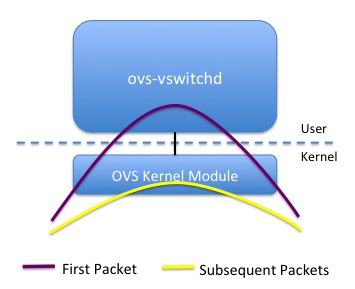
\includegraphics[scale=0.65]{ovs_dataplane}
	\centering
	\label{fig:ovs_dataplane}
\end{figure}

\subsection{RAUController}
En el uso típico de Mininet, la comunicación entre el controlador y el switch se da a través de la interfaz de loopback. Esto es así porque los switches no tienen su propio namespace. Para lograr dicha comunicación, no hace falta un objeto en Mininet que represente el controlador, ya que ejecutar la aplicación en el sistema operativo base ya habilita al switch a comunicarse con ella a través de la interfaz de loopback. Esta situación cambia en este diseño, porque los switches pasan a tener su propio network namespace. Esto lleva a la necesidad de crear un host virtual, que ejecute la aplicación de RAUFlow y se comunique con los switches a través de enlaces virtuales. Para satisfacer esta necesidad se usa la clase RAUController.

\subsection{QuaggaRouter}
Es una clase similar al RAUSwitch pero sin Open vSwitch, es decir, sólo usa Quagga. Apunta a representar el router CE que utilizaría una subred para conectarse a la red. Está conectado a un RAUSwitch de borde.

\subsection{RAUHost}
Representa a los hosts que serán clientes de la red. Con este propósito, se podría utilizar directamente la clase Host de Mininet, pero se construye esta clase auxiliar para evitar determinadas configuraciones manuales, como por ejemplo, el \textit{default gateway}.

\subsection{Sustitución del agente SNMP}
Como se explicó en el capítulo (X), RAUFlow usa un agente SNMP en cada switch para hacer disponible al controlador, información acerca de sus interfaces de red que no puede enviar a través de OpenFlow. Específicamente, los datos que se envían a través de SNMP para cada interfaz de red son dirección IP, dirección MAC y nombre de interfaz. Para lograr esto en el entorno virtual se debe crear una instancia de agente SNMP por cada RAUSwitch virtual que se ejecuta, y se las debe configurar de tal forma para que cada una sólo devuelva la información de su nodo virtual. \\
Si bien es posible, se observa que lograr esto es relativamente complejo, debido que se aleja mucho del uso tradicional de SNMP. A esto se suma el hecho de que si bien es necesario que esa información llegue al controlador de alguna forma, no es estrictamente necesario que sea mediante SNMP. Por lo tanto, se concluye que la información que RAUFlow envía al controlador a través de SNMP, sea enviada de otra forma en el entorno virtual.

La alternativa que se construye está basada en Open vSwitch. Mediante el comando 'ovs-vsctl list bridge', se pueden ver las distintas propiedades del switch, como el identificador de datapath, estado, etc. Entre esas propiedades, existe un campo llamado 'other\_config', al que se le pueden agregar un número de configuraciones adicionales. Entonces, se utiliza ese campo para almacenar una propiedad llamada 'ports\_info' que almacenará la información sobre todas las interfaces del nodo. Esta propiedad no tendrá significado para Open vSwitch, por lo tanto quedará intacta. El valor que almacenará la propiedad debe ser de tipo String, y probablemente almacene la información de múltiples interfaces de red, así que se debe crear un formato para esa información. Por ejemplo, si tenemos un switch con la siguiente información:
\begin{lstlisting}
Interfaz de red 1:
	Nombre: eth1
	Direccion IP: 10.0.0.1
	Direccion MAC: 00:00:00:00:00:01
Interfaz de red 2:
	Nombre: eth2
	Direccion IP: 10.0.0.2
	Direccion MAC: 00:00:00:00:00:02
\end{lstlisting}
El valor de ports\_info sería el siguiente:
\begin{lstlisting}
eth1_10.0.0.1_00:00:00:00:00:01/eth2_10.0.0.2_00:00:00:00:00:02
\end{lstlisting}

Como se puede ver, el formato indica que se usa el carácter '/' para separar la información de cada interfaz, y el carácter '\_' para dividir los campos de información de cada interfaz. Este formato no es el único posible, se puede utilizar cualquier otro siempre y cuando use los caracteres permitidos por Open vSwitch.

Después de configurar el campo ports\_info, cada instancia de Open vSwitch almacena la información de las interfaces de su respectivo nodo virtual. Sin embargo, esta información todavía no es accesible desde afuera del nodo. Para lograr que Open vSwitch pueda enviar esta información por la red, se utiliza un comando llamado 'set-manager'. Con él, se le puede indicar a Open vSwitch que escuche en un determinado puerto (típicamente el puerto TCP 6640) para que pueda ser gestionado de forma remota. Por lo tanto, si el controlador desea saber los datos de las interfaces de un determinado switch, alcanza con que le envíe el comando 'ovs-vsctl list bridge' a través de la red y parsear la respuesta para extraer los datos de interés.

Como se explicó anteriormente, esta alternativa se construye para evitar la adaptación de SNMP al entorno virtual. Sin embargo, se considera que es una buena solución al problema de los datos de las interfaces. En primer lugar, la arquitectura se simplifica, ya que elimina la necesidad de SNMP. Esta solución utiliza aspectos de Open vSwitch, que ya está integrada a la arquitectura, por lo que no agrega mucha complejidad. En segundo lugar, eliminar la necesidad de que cada nodo ejecute un agente SNMP ayuda a la performance de los mismos. Por estas razones, se sugiere esta solución como aporte a RAUFlow.

\section{Módulo de carga automática - GraphML Loader}
Como se explica en el Apéndice 1, cada topología se debe configurar en un script Python usando la API del entorno. Este proceso puede ser tedioso, especialmente si se trata de una topología grande. Todos los nodos se deben inicializar con los parámetros que requieren, también se deben crear los enlaces entre ellos, y cualquier problema de coherencia en los datos puede resultar en un funcionamiento inadecuado de la topología.

Tomando como base \cite{auto-mininet}, se desarrolló un módulo llamado \textbf{GraphML Loader}. Su propósito es facilitar la tarea de configurar topologias nuevas. GraphML es un formato de archivo que sirve para detallar grafos (sus nodos, enlaces, etc), y está basado en XML. Este formato es usado, por ejemplo, en el dataset de Topology Zoo \cite{topology-zoo} para detallar las topologias. El propósito de este módulo es recibir como entrada un archivo de tipo graphml y producir como salida un script Python que configura la topología que se corresponde con el grafo de entrada. El módulo se encarga no sólo de crear una topología que se adapte al grafo, sino que también de asignar automáticamente las direcciones IP de cada nodo, indicar qué nodos son de borde y cuales no, entre muchas otras cosas. Este módulo aporta una gran mejora a la usabilidad del entorno virtual, ya que si el usuario dispone de un archivo de tipo graphml, puede tener una topología lista para usarse en pocos segundos. En caso que se desee hacer una modificación a dicha topología, alcanza con hacerla en el script que produjo el módulo. En el Apéndice 2 se explica más detalladamente como funciona este componente.

\section{Verificación funcional del entorno virtual}
\subsection{Escenario 1}
En este escenario se crea una VPN punto a punto de capa 3 entre las dos subredes cliente, y se controla que tanto la creación de la VPN como el uso de la misma con tráfico, funciona correctamente. Esto se repite para cada topología de prueba. Los puntos específicos que se busca verificar se detallan a continuación: \\ \\
\textbf{Algoritmo de ruteo} \\
Se verifican dos aspectos claves: que el camino se corresponde con el camino esperado (calculado previamente de forma manual), y que el camino es correctamente instalado en forma de reglas de reenvío (en base a conmutación de etiquetas MPLS) en las respectivas tablas de flujos OpenFlow de cada nodo del camino. Todo esto se puede comprobar analizando las tablas de flujos de cada nodo, que se pueden ver utilizando el comando \textbf{dump-flows} de Open vSwitch. También se puede utilizar la interfaz gráfica de RAUFlow, aunque no se recomienda su uso con topologias grandes (como pueden ser la mediana o grande, en este caso) ya que la forma de presentar los nodos se vuelve demasiado caótica. Desde las tablas de flujos se puede reconstruir el camino que computó la aplicación, y también comprobar que los flujos manipulan correctamente las etiquetas MPLS. \\ \\
\textbf{Clasificación de tráfico} \\
La idea es verificar que realmente se están asignando las etiquetas MPLS al tráfico entrante, así como comprobar que el mismo es reenviado por los nodos correctos. Para probar esto se utilizará una VPN de capa 3, que permitirá tráfico con ethertype 0x0800, es decir, del protocolo IPv4. Se generará tráfico de este tipo utilizando el comando \textbf{ping} y la herramienta \textbf{iperf}. Con la herramienta tcpdump, se verificará que el tráfico pasa correctamente por cada nodo del camino. \\

\begin{table}[ht]
	\caption{Pasos que cumple cada caso en la creación y uso exitoso de un servicio.}
	\centering 
	\resizebox{\textwidth}{!}{%
		\begin{tabular}{c c c c c}
			\hline\hline
			Largo del camino (topología) & Servicio & Camino & Flujos  & Clasificación de tráfico \\ [0.5ex]
			\hline
			1 (básica) & X & X & X & X \\
			7 (chica) & X & X &  &  \\
			10 (mediana) &  &  &  &  \\
			12 (grande) &  &  &  &  \\ [1ex]
			\hline
		\end{tabular}
	}
	\label{table:problemas_por_topologia}
\end{table}

Con el propósito de hacer un diagnóstico más preciso sobre el proceso de creación y uso de una VPN, se lo descompone de 4 pasos conceptuales en los cuales podría haber fallas. Estos pasos son: (a) se crea con éxito el servicio, (b) el camino que se calcula es correcto, (c) los flujos de cada nodo del camino son correctos, (d) se clasifica correctamente el tráfico. Si se cumplen los 3 primeros pasos quiere decir que el servicio (y por ende la VPN que lo utilice) se establece correctamente y si se cumple el último paso entonces el tráfico pasa sin problemas por el servicio creado. En la tabla \ref{table:problemas_por_topologia} se detallan los comportamientos observados para algunos de los casos estudiados. En ella se indica con una X los pasos que funcionaron correctamente para cada caso. Las celdas vacías indican qué paso falló en cada caso. \\

Analizando la tabla \ref{table:problemas_por_topologia} se pueden observar como mínimo dos problemas. El primero es que en el caso de la topología chica y un camino de 7 saltos, el servicio se crea y los flujos están en los nodos correctos (los del camino más corto entre las subredes cliente), pero los mismos no son correctos. El segundo comportamiento que se observa es que para el caso del camino de 10 saltos en la topología mediana, y el de 12 saltos en la topología grande, el servicio ni siquiera llega a crearse correctamente, es decir, la aplicación sufre una excepción de Python al intentar hacerlo. Las razones que explican esto, así como sus respectivas soluciones (si son posibles) se encuentran en la anterior sección 3.5, donde se explican los problemas encontrados y/o resueltos en el entorno. El resto de las pruebas que se mencionan en este capítulo fueron realizadas con dichas correcciones ya hechas.

\section{Problemas y errores encontrados}
Como resultado de las pruebas funcionales básicas que se efectuaron sobre el entorno (que son detalladas en la sección 4.1.1) se detectaron determinados problemas que fueron necesarios estudiar. Esta sección explicará en que consiste cada problema, estudiando sus síntomas, su explicación, y en caso de que exista una, su solución. Como se verá, algunos de ellos se manifestarían en un despliegue real de la arquitectura, y otros son a causa del uso de un entorno virtual, y por lo tanto no se deberían tener en cuenta en un despliegue real.

\subsection{Errores en el código de RAUFlow}
Se descubrió que existían determinados errores (o "bugs") en el código de RAUFlow. Como son errores en el código del controlador, es importante remarcar que estos errores sin lugar a dudas se manifestarían en una red real. \\ \\
\textbf{Error en flujos de servicio con más de un salto} \\
\begin{figure}[t]
	\caption{Escenario donde los flujos están mal configurados. Muestra la topología de la red y los flujos de interés para cada nodo.}
	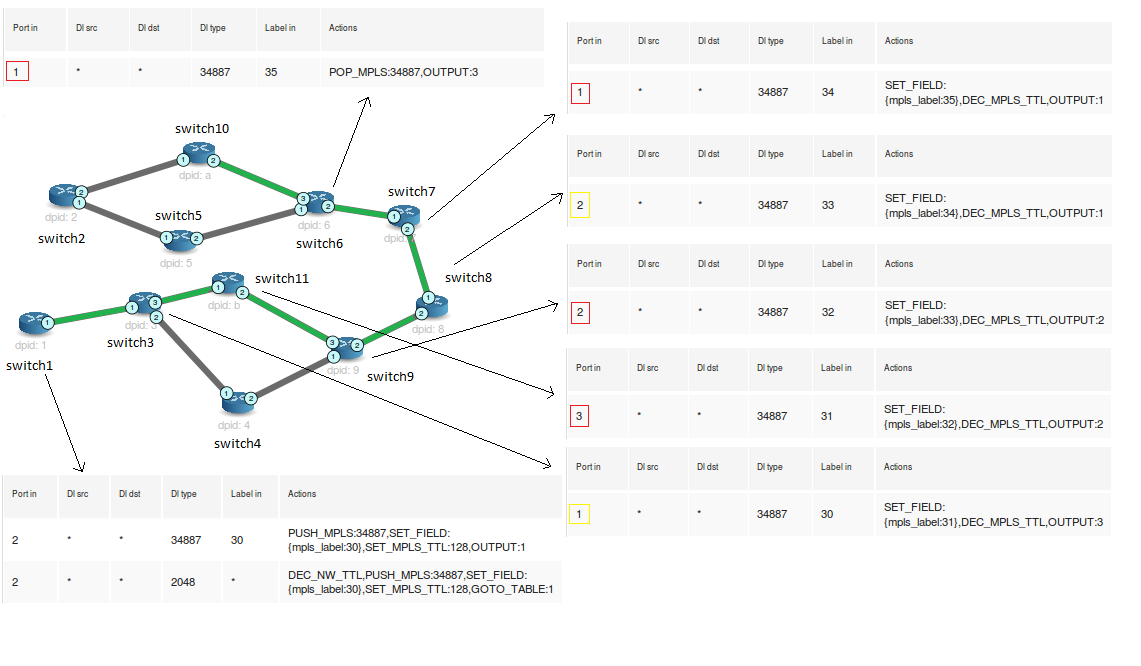
\includegraphics[scale=0.5]{flujos_incorrectos}
	\centering
	\label{fig:flujos_incorrectos}
\end{figure}
Se observó que cuando se trataba de crear un servicio que pasara por más de 2 nodos (es decir, con más de un salto), el controlador instalaba flujos en los nodos correctos, pero los flujos mismos no eran correctos. Esto indicó que el problema no se encontraba en el algoritmo de ruteo, sino que en el algoritmo encargado de configurar los flujos en cada nodo del camino computado. Específicamente, el problema es que los flujos en los nodos intermedios (es decir, los nodos donde no empieza ni termina el servicio) tenían un incorrecto puerto de entrada. En la figura \ref{fig:flujos_incorrectos} se examina este comportamiento. Los enlaces verdes muestran el camino del servicio que se intentó crear, y cada flecha indica la tabla de flujos (reducida) de cada nodo relevante. Si se presta atención a los flujos en los nodos intermedios, se puede ver que los puertos de entrada de cada flujo coinciden con el puerto de salida del flujo en el nodo anterior. Los recuadros rojos muestran los puertos incorrectos y los amarillos indican los que podrían haber sido incorrectos pero no lo son por coincidencia.
Para solucionar esto se creó un "fork"\footnote{https://github.com/santiagovidal/LiveCode} del repositorio de RAUFlow, y se hizo el commit\footnote{https://github.com/santiagovidal/LiveCode/commit/aeb575a10eb241dc3980a4c37846af7551bb7060} correspondiente. \\ \\
\textbf{Error de tipos en el algoritmo de ruteo} \\
Se detectó que al intentar crear servicios en algunas topologias, se producía un error 500 de Python en RAUFlow. Luego de inspeccionar el código se concluyó que el problema radicaba en la implementación del algoritmo de ruteo, que está basado en Dijkstra. En el proceso de calcular el camino óptimo, el algoritmo de Dijkstra acumula iterativamente los costos desde el origen hasta los nodos intermedios. Dado que los costos de cada enlace son números enteros, la acumulación de costos debería implementarse simplemente aplicando suma entera a dichos costos. Sin embargo, la estructura interna usada para representar el grafo, almacena los costos de cada enlace con tipo "String". Al hacer la suma para acumular los costos, en vez de aplicar suma entera, el código hacía concatenación de strings. Dada la estructura interna del código, que no se mencionará para simplificar, esto generaba un error 500 sólo en algunas topologias. Para solucionar esto se realizó un casteo de String a Int en el código del algoritmo. Al igual que en el error mencionado en el punto anterior, se realizó un commit\footnote{https://github.com/santiagovidal/LiveCode/commit/4128923efcff38768aefd2864e10bd1adb63df52} con dicho arreglo. \\ \\

\subsection{Problemas de comunicación con muchos nodos}
Cuando se iniciaba el entorno con una topología grande, de unos 100 nodos aproximadamente, ocurría que al principio los nodos se registraban correctamente con el controlador y la comunicación parecía ser la esperada, pero luego de unos segundos el controlador anunciaba que los nodos se habían desconectado.
Igual que el prototipo físico, el entorno virtual necesita que cada topología también defina una red de gestión para que el controlador pueda comunicarse con los nodos en modo out-of-band. Dado que era probable que el problema se encontrara en dicha red, se utilizó la herramienta Wireshark (un analizador de protocolos ampliamente usado) para monitorear la comunicación entre los nodos y el controlador. Si la comunicación es correcta, se debería ver algo como lo que muestra la figura \ref{fig:openflow_protocol}. Luego del 'handshake' inicial, se entra en un ciclo en el que el switch envía un mensaje llamado Echo Request al controlador y espera la respuesta Echo Reply del mismo. Cuando se recibe dicha respuesta se empieza de nuevo el ciclo. \\
Sin embargo, lo que en realidad se observa en Wireshark se indica en la figura \ref{fig:openflow_protocol_error}. El handshake se efectúa correctamente, y cuando se inicia el ciclo de Echo Request - Echo Reply, en algún punto el controlador no responde, o demora demasiado en mandar la respuesta. En la figura se muestra que eso ocurre con el primer Echo Request, pero no necesariamente es el caso en la práctica. Cuando el switch detecta que pasó demasiado tiempo esperando la respuesta a su Echo Request, asume que la conexión se ha finalizado y envía de nuevo mensajes Hello para intentar volver a conectarse. \\
\begin{figure}[t]
	\caption{Protocolo de control de OpenFlow.}
	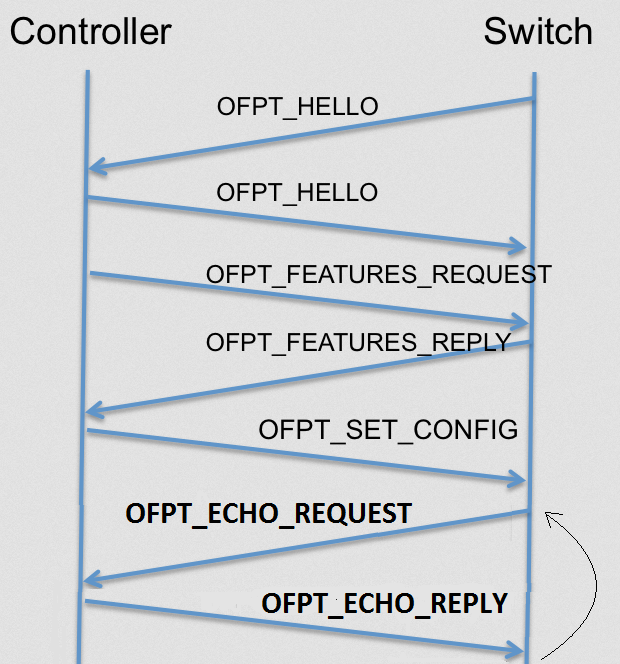
\includegraphics[scale=0.5]{openflow_protocol}
	\centering
	\label{fig:openflow_protocol}
\end{figure}

\begin{figure}[t]
	\caption{Error de comunicación en protocolo de OpenFlow.}
	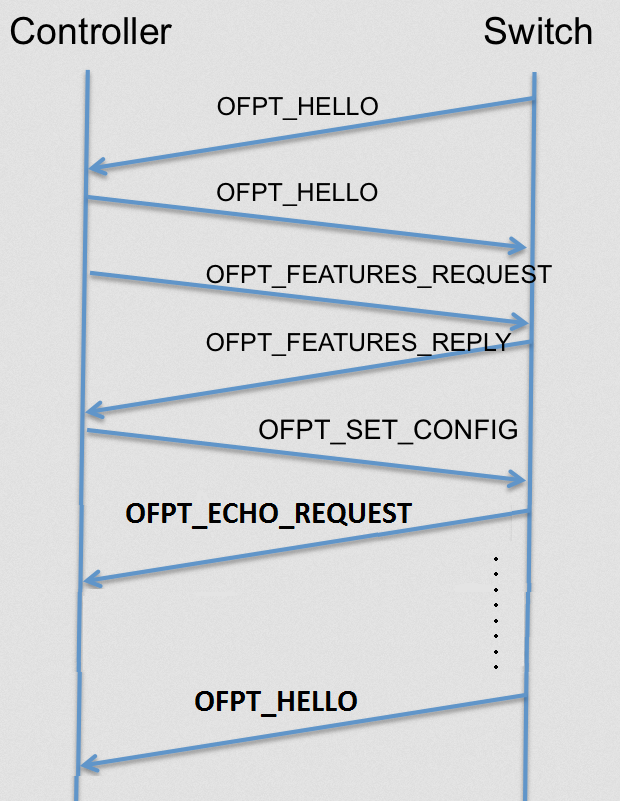
\includegraphics[scale=0.5]{openflow_protocol_error}
	\centering
	\label{fig:openflow_protocol_error}
\end{figure}
De acuerdo al manual de Open vSwitch \cite{ovs-vswitchd-conf}, la variable responsable de este comportamiento es la llamada \textbf{inactivity\_probe}. Se define como el máximo número de mili-segundos que debe esperar el switch antes de enviar un mensaje sonda por inactividad (Echo Request). Si Open vSwitch no se comunica con el controlador por la cantidad especificada de segundos, enviará una sonda, es decir, un mensaje Echo Request. Si la respuesta no es recibida dentro la misma cantidad de mili-segundos adicional, Open vSwitch asume que la conexión se ha finalizado e intenta reconectarse. El valor por defecto para esta variable depende de la implementación, y en el ambiente de trabajo tiene por defecto el número 5000 (5 segundos). Esto quiere decir que si el switch no recibe mensajes del controlador por 10 segundos (5 luego de mandar la sonda) se cerrará la conexión. \\
Lo interesante de esta situación es estudiar por qué el controlador no logra responder a tiempo las sondas de los nodos. Algunas posibles razones son las siguientes:
\begin{itemize}
	\item Congestión en la red de gestión. Es posible que el exceso de nodos genere demasiado tráfico de control, y por ende haya retrasos y/o pérdidas en la red de gestión. Este problema posiblemente estaría presente en un despliegue real de la arquitectura.
	\item Falta de capacidad de cómputo. Dado que este comportamiento se detectó en el entorno virtual y con un número importante de nodos, es posible que el controlador no tenga acceso al poder de cómputo suficiente como para responder a tiempo a todas las sondas. Este sería un problema del entorno virtual, y no sería relevante en una red real.
	\item Incapacidad de Ryu para manejar muchos nodos. En \cite{proyecto-rrap} se menciona que Ryu es un controlador minimalista y académico. Por lo tanto, es posible que no esté diseñado para controlar tantos switches. Si ese fuera el caso, esto sería un obstáculo al desplegar la arquitectura en una red real. TODO!: Mencionar CBench o otro benchmark para controllers como posible manera de analizar.
\end{itemize}
Como solución provisoria, con el propósito de realizar pruebas con las topologias que presentan este problema, se configuró el valor de inactivity\_probe como un número muy alto (45 segundos) de modo de darle al controlador más que suficiente tiempo para responder a las sondas. Sin embargo, esta no es una buena solución ya que en una red real, cuanto más alto esté ese número, más demoraría el controlador en darse cuenta que un switch se desconectó. Se deja para trabajos futuros investigar si esto podría afectar una despliegue real, ya que si lo hace, tendrían que hacerse cambios radicales a la arquitectura.

\subsection{Problema de concurrencia por muchas instancias de OpenVSwitch}
Como se explica en el Proyecto RRAP \cite{proyecto-rrap}, para que las interfaces de red de los nodos funcionen como puertos OpenFlow con dirección IP, no solo se debe crear un puerto en Open vSwitch para cada una, sino que también se debe crear una interfaz virtual con su respectivo puerto. Además, deben crearse flujos para que los paquetes que entran por la interfaz física salgan por su respectiva interfaz virtual, y viceversa.
El siguiente código simplificado muestra como es el proceso de configuración:
\begin{lstlisting}
	ovs-vsctl add-port eth0		#deberia asignar nro de puerto OF 1
	ovs-vsctl add-port eth1		#deberia asignar nro de puerto OF 2
	ovs-vsctl add-port eth2		#deberia asignar nro de puerto OF 3
	ovs-vsctl add-port veth0	#deberia asignar nro de puerto OF 4
	ovs-vsctl add-port veth1	#deberia asignar nro de puerto OF 5
	ovs-vsctl add-port veth2	#deberia asignar nro de puerto OF 6
	
	ovs-ofctl add-flow in_port=1,output:4
	ovs-ofctl add-flow in_port=4,output:1
	ovs-ofctl add-flow in_port=2,output:5
	ovs-ofctl add-flow in_port=5,output:2
	ovs-ofctl add-flow in_port=3,output:6
	ovs-ofctl add-flow in_port=6,output:3
\end{lstlisting}
Cuando se le agrega un puerto, Open vSwitch le asigna automáticamente un número de puerto OpenFlow. La manera en que Open vSwitch hace esa numeración es secuencial, empezando desde 1. Eso quiere decir que, en teoría, si se agregan 3 puertos a Open vSwitch, sus puertos OpenFlow tendrán los números 1, 2 y 3, de acuerdo al orden en que fueron creados. Como se ve en el pseudocódigo, las líneas que agregan los flujos que \enquote{conectan} las interfaces virtuales y físicas asumen que la numeración se hace de esa forma. Está configuración se hace para cada nodo (es decir, para cada instancia de Open vSwitch) y es equivalente a la forma en que se configuran los dispositivos físicos en el prototipo. \\
No se observaron problemas relacionados con esto en topologias chicas de 4 nodos aproximadamente, pero sí en topologias más grandes. Se observó que con más nodos, la numeración de los puertos en Open vSwitch se comportaba de forma impredecible, y no seguía el esquema secuencial que se mencionó anteriormente. Como los flujos que se agregan posteriormente asumen ese determinado orden, eso causa que varias o todas las interfaces del nodo no funcionen. En topologias de entre 10 y 40 nodos ese comportamiento a veces afectaba sólo unos pocos nodos, y en ocasiones no ocurría. Con topologias de 100 nodos aproximadamente, esto ocurría siempre, con más de la mitad de los nodos. Esto llevó a creer que se trataba de un problema de concurrencia por tener muchas instancias de Open vSwitch iniciándose y configurándose al mismo tiempo. \\
Para solucionar este problema se hizo el siguiente cambio:
\begin{lstlisting}
	ovs-vsctl add-port eth0 ofport_request=1
	ovs-vsctl add-port eth1 ofport_request=2
	ovs-vsctl add-port eth2 ofport_request=3
	ovs-vsctl add-port veth0 ofport_request=4
	ovs-vsctl add-port veth1 ofport_request=5
	ovs-vsctl add-port veth2 ofport_request=6
	
	ovs-ofctl add-flow in_port=1,output:4
	ovs-ofctl add-flow in_port=4,output:1
	ovs-ofctl add-flow in_port=2,output:5
	ovs-ofctl add-flow in_port=5,output:2
	ovs-ofctl add-flow in_port=3,output:6
	ovs-ofctl add-flow in_port=6,output:3
\end{lstlisting}
El parámetro opcional \textbf{ofport\_request} permite indicarle a Open vSwitch que número debería asignarle al puerto que se está agregando. Esto soluciona completamente el problema y permite levantar topologias de cualquier tamaño sin problemas. Es importante remarcar que probablemente esto solo afecta al entorno virtual, y no es necesario realizar esta corrección al configurar nodos reales, ya que cada dispositivo ejecuta una única instancia de Open vSwitch y por lo tanto no es probable que se vea este comportamiento. Sin embargo, no se descarta del todo que exista una posibilidad de que esto ocurra, así que se propone el uso de \textbf{ofport\_request} para la configuración de los nodos físicos para eliminar ese riesgo, por más pequeño que sea.

\subsection{Problema de LSDB Sync con muchos nodos}
Como se explicó en el capítulo X, el componente llamado LSDB Sync es el encargado de procesar la información de la base de datos topológica de OSPF y enviarla a las aplicaciones que se ejecutan en el controlador. Este proceso se lleva a cabo en un script escrito en Python, el cual se conecta mediante Telnet con el demonio OSPF, extrae la información topológica y la procesa, y luego la envía al controlador. Se observó que si se está simulando una topología grande (de 100 nodos aproximadamente), la ejecución de este script queda colgada, y no termina. Por lo tanto, la información no se envía nunca al controlador. Para explicar la fuente del problema, es necesario mostrar un pseudocódigo del script:
\begin{lstlisting}
conexion = telnetlib.iniciar_conexion("localhost", PUERTO_OSPFD)
conexion.write(password)
conexion.write("show ip ospf database router")
conexion.write("exit")
info_topologica = conexion.read_all()

procesar_info_topologica
enviar_info_controlador
\end{lstlisting}
La tarea de conectarse con el demonio OSPF mediante Telnet y extraer la información topológica se hace con una librería llamada Telnetlib. La parte que se observó era problemática es la llamada al método \textbf{read\_all()}, usada para leer la información que devuelve el demonio. Al existir muchos nodos, la cantidad de información que deberá devolver el método será extensiva. Se calcula que para topologias de 100 nodos aproximadamente, esa información ronda los 92KB. Aunque no se encontró documentación que lo soporte, el diagnóstico que se hizo es que dicho método no está diseñado para devolver tanta información, y quizás queda colgado por limitaciones de memoria o buffers.

A diferencia de read\_all, que se bloquea hasta terminar de leer, el método \textbf{read\_very\_eager()} lee toda la información que puede pero sin bloquearse \cite{doc-telnetlib}. Con el segundo método, el script no se cuelga, pero sí devuelve información incompleta en ocasiones. Por lo tanto, se adoptó read\_very\_eager como solución al problema, y se agregó una validación al script que compruebe que la información no está incompleta antes de enviarla al controlador.

Se propone un estudio más profundo sobre este tema para trabajos futuros por dos razones. En primer lugar, no se conoce con certeza la razón del comportamiento, y la solución que se adopta lo resuelve pero parcialmente. En segundo lugar, este defecto podría afectar a despliegues reales de la arquitectura RAUFlow.

\subsection{Precaución con MTU}
A diferencia de los problemas mencionados en las secciones anteriores, en esta sección no se discutirá un problema de la arquitectura ni del entorno virtual, sino de una precaución que se debe tener en cuenta a futuro. Como se explica en el capítulo X, las VPN se implementan agregando y quitando etiquetas MPLS a los paquetes que pasan por los switches. Esas etiquetas son de 5 bytes, y dependiendo el camino que debe recorrer, a un paquete se le puede agregar una o dos etiquetas. Es importante tener esto en cuenta ya que impacta en el MTU. Por ejemplo, si se tiene una red Ethernet con un MTU de 1500 bytes, y se envía tráfico TCP sin tener esto en consideración, probablemente se utilice un MSS (Maximum Segment Size) de 1460 bytes, dejando 20 bytes para el cabezal IP y 20 más para el TCP. En ese caso, el tráfico no pasa por la red, ya que cuando el switch de borde recibe los paquetes y les asigna las etiquetas MPLS que corresponden, los mismos pasan a tener más de 1500 bytes, y por lo tanto no se envían. Para solucionarlo, se debe reducir el MSS a 1455 en caso de que el camino sea de un salto (se le asigna una etiqueta), y a 1450 en caso contrario (se asignan dos etiquetas).
